\documentclass[border=2mm]{standalone}
\usepackage{tikz}
\usetikzlibrary{arrows,shapes,snakes,automata,backgrounds,petri,matrix}

\begin{document}
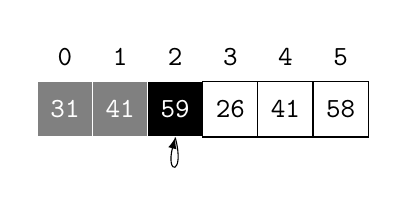
\begin{tikzpicture}[
font=\ttfamily, array/.style={
    matrix of nodes, 
    nodes={draw=black, minimum size=7mm},
    column sep=-\pgflinewidth, 
    row sep=0.5mm, 
    nodes in empty cells,
    row 1/.style={ nodes={draw=white, fill=none, minimum size=5mm}},
    row 1 column 1/.style={nodes={draw}},
},
    bend angle=80,
    out=60,
    in=30,
    pre/.style={<-,shorten <=1pt,>=stealth,semithick},
    post/.style={->,shorten >=1pt,>=stealth,semithick},
    outer sep = auto
]

\matrix[array] (array) {
  0  &  1  &  2  &  3  &  4  &  5  \\
  |[white, fill=gray]|31 &  |[white,fill=gray]|41 & |[white,fill=black]| 59 &  26 & 41  & 58  \\
};

\draw[-latex] (array-2-3.south) to[loop below] (array-2-3.south);

%
\end{tikzpicture}
\end{document}
